\section{Deployment\label{deployment_methods}}

In this section, a comprehensive description of tools, resources and the architecture for deploying the \acrshort{ml} model is discussed. There are number of ways to deploy \acrshort{ml} systems, for instance hosting a server locally that is having an endpoint from where user can access the model. However, hosting a model from a local server means more maintenance and costs. Front investment for a server and installation in addition with maintaining such infrastructure adds more costs making it a critical factor in small scale industries. Moreover, the question of security still remains since it is difficult to achieve robust protection of the resources. Cloud technology can be a good solution in this case, generally cloud providers provides functionalities such as scalability, flexibility, security, disaster recovery and so on that can take the front investment and maintaining costs from these small scale industries resulting less cost for them to have access to a good computing power. 

Our aim is to make model available for the end-user in a way that is scalable, secure, fast and user's does not require to download or install any dependencies in terms of consuming it. In order to achieve this we have used cloud provider \acrfull{aws}\footnote{\url{https://aws.amazon.com/free/}, Accessed: 19.04.2024} as an infrastructure provider. \acrshort{aws} provides around 200 services that includes compute, storage, databases, analytics, networking, developer tools, management tools, \acrshort{iot} and so on. When it comes to providing \acrshort{ml} services, compute, networking and storage are the prime factors that needs to be handle carefully. \acrshort{ml} models are large itself and training of these models requires high-performance compute resources in addition with a requirement of storing the datasets. On other hand to develop an inference for the model have their own requirements and challenges, for instance once the model is ready to use, we have to think of different networking aspects like inter-node communication and scalability of the complete system in order to provide ML as a service. \acrshort{ec2} is a IaaS type of service that is broadest and deepest compute platform provided by AWS. It is also refers as an instance and \acrshort{aws} provides over 750 different types of instances to meet the demand and need of the user in terms of processor, storage, networking, operating system and so on. For storage, \acrshort{aws} provides \acrfull{s3}\footnote{\url{https://aws.amazon.com/s3/},Accessed:19.04.2024 \label{s3}}, which organizations of all sizes, across different industries can use to make their data lakes to transform and manage the assets. In addition, \acrshort{aws} support all ML frameworks such as Tensorflow\footnote{\url{https://www.tensorflow.org/}, Accessed: 22.04.2024}, PyTorch\footnote{\url{https://pytorch.org/}, Accessed: 22.04.2024}, Keras\footnote{\url{https://keras.io/}, Accessed: 22.04.2024} and so on. These \acrshort{ml} frameworks helps in various ML tasks from building a model to deployment. It provides useful and complex various ML  algorithms and make them easy to use and implement to deal with tasks such as time series, natural language processing and computer vision. Moreover, \acrshort{aws} provides workflow services like Amazon SageMaker\footnote{\url{https://aws.amazon.com/sagemaker/}, Accessed: 22.04.2024 \label{sagemaker}}, Deep Learning Containers\footnote{\url{https://github.com/aws/deep-learning-containers}, Accessed: 22.04.2024 \label{deepcontainer}}, Elastic Kubernetes service\footnote{\url{https://aws.amazon.com/eks/}, Accessed: 22.04.2024 \label{eks}}, Elastic Container Service\footnote{\url{https://aws.amazon.com/ecs/}, Accessed: 22.04.2024 \label{ecs}} and so on. Services like SageMaker\(^{\ref{sagemaker}}\), provides tools like notebooks, debuggers, pipelines, MLOps and so on to build, train and deploy the \acrshort{ml} models at scale. On other hand,  containerization services\(^{\ref{deepcontainer}, \ref{eks}, \ref{ecs}}\) help removing the burden of operating system dependency from the system by making system a self-contained environment, which allows the application to run independently from hosted operating systems. 

We have tried to use few infrastructures, frameworks and workflow services in order to find and develop a suitable cloud infrastructure to serve a ML model as a SaaS product for scalable solution. In addition, in order to make the service scalable, serverless and independent from the hosted and individuals operating systems, we will use \acrshort{aws} Lambda services\footnote{\url{https://aws.amazon.com/lambda/}, Accessed: 22.04.20274 \label{lambda}} in combination with containerization approach. A comprehensive description of few important terms to develop cloud architecture is described below. 

\subsubsection{Frontend and Backend}
Frontend and backend are two critical parts of any software or application. The frontend refers to the graphical user interface (GUI) that users can see and interact with. Usually frontend includes visual elements like check-boxes, graphics, buttons, text messages, navigation menus and so on. Traditionally, \acrfull{html} is being used to define the frontend structure and different elements, later on \acrfull{css} and JavaScript started grasping the way these HTML document is defined. Currently, CSS and JavaScript became an important part to define the style of a web application such as layout, fonts, colors, visual style and dynamic functionality. 

On other hand, backend is responsible for overall functionality of the application. whenever the users interacts with the frontend, this interaction sends a request to the backend (usually HTTP format), the backend process the request and returns a response. Backend processes can be a request to a database to serve the retrieval or modified data, Microservices that performs some predefined task, a third-party APIs to collect some additional information or to perform additional functions.


\subsubsection{Application Programming Interface (API)}
An \acrshort{api} is a set of rules or protocols, through two or more computer programs or various components can communicate with each other in terms of exchanging data, features and functionality.  \acrshort{api} stands for application programming interface where the word application denotes any software with a function. Interface is a contract of service between any two application of software, where these contracts set the boundary how this two component should interact with each other using request and responses (Event). The architecture of the \acrshort{api} can be explained in terms of client and server. The application making a request becomes the client and one receiving this request becomes the server. Traditionally, \acrfull{http} were used to communicate between web clients and servers over internet (\acrshort{www}). \acrshort{https} is the secure version of \acrshort{http}, it encrypts the payload using protocols such as transport layer security(TLS) in order to increase the security of data transfer. Restful APIs or Rest APIs and Websocket APIs are well known type of APIs. These type of \acrshort{api}s are optimized versions of \acrshort{https} \acrshort{api}s, that offers enabling real-time two-way communication in application. In addition, developers can secure the \acrshort{api}s using different authentication layers. For instance, Authentication tokens and API keys are used to authorize users to make a call to \acrshort{api}s by checking whether the users are who they claim to be and have access rights to call. \acrshort{aws} also provides managed service \acrshort{api} Gateway\footnote{\url{https://aws.amazon.com/api-gateway/}, Accessed: 23.04.2024 \label{api_gateway}}, It helps developers to create, publish, maintain, monitor and secure \acrshort{api}s. 




\subsubsection{Containerization}
Traditionally, in order to run any application on any machine, we need to install all the dependencies, libraries including the version that requires by the operating systems. Containerization is a process used in software deployment, the basic fundamental of it is to bundle the application's code including all the dependency that requires to run the application, libraries, files and so on into one software package that also known as a container. This container have their own operating system and on top of this the application along with all dependency and libraries can be installed. Once the container is ready than one can use the application by just running the container and it will work on all types of devices and operating systems. Containerization approach helped to increase portability, scalability, fault tolerance and agility into the software deployment process. The process to make this container in the executable file refers to image or container image. These container images can be stored on a hub with all the necessary libraries, dependencies and files that the container needs to run and different component or users can access to the application or functions that is stored under these container images. Amazon \acrfull{ecr} is a managed registry provided by aws, one can push and pull the container images without installing or scaling infrastructure using management tools to store, share and deploy the containerized applications using \acrfull{https}. 

\subsubsection{AWS Lambda}
Lambda\(^{\ref{lambda}}\) is a compute service that triggers or initiates with an event and runs a code in order to provide response, that helps to make an idea into a modern, production and serverless applications quickly.  An event is a JSON-formatted document that contains the data to be process. There are few advantages of using AWS Lambda such as running code without provisioning or managing infrastructure, Scripts can be write and uploaded as a .zip file or container image. In addition, Lambda responds to the coming request and scale it from dozen of events per day to hundreds of thousands per second. Moreover, one can optimize the code execution time and performance with correct amount of allocating memory size to lambda function and reduce the respond time to milliseconds. The upper hands of Lambda like concurrency(ability to scale up) when the demand is high and scale it down to zero when there is no request pending makes Lambda a powerful way to deploy the scalable applications faster and cheaper. 

\subsection{Using S3-Bucket for triggering the containerized Lambda \label{s3_deployment}}

In \Cref{fig:s3-trigger-workflow}, a simple workflow to deploy the \acrshort{ml} model is shown. In this approach the user initiate the workflow by simply uploading the document to the S3\(^{\ref{s3}}\) Bucket. The word bucket refers to a container for objects that are stored in S3. These S3 buckets comes with a functionality to add a trigger that can be configure. For this workflow, we have configured a trigger for each time the user is uploading a document into the bucket. This trigger will initiate the event in order to invoke the lambda function. The lambda function will then pull the container image from the \acrshort{ecr} that is having the application's code and all the dependencies installed in the container itself including the \acrshort{ml} model. Currently Lambda supports 10GB of container image size and since the base model of \acrshort{lilt} was around 3GB it was possible to store the model on a container image. As the applications needs libraries and dependencies to be installed in order to use the model and it was not possible to store any of \acrshort{ocr} engine into the container image itself without exceeding the size limit of 10GB. Therefore, once the lambda function is deployed using the container image with our \acrshort{ml} model, it will pass the document received from the user to Amazon Textrect\footnote{\url{https://aws.amazon.com/textract/}, Accessed: 22.04.2024 \label{textract}} which is a \acrshort{ocr} based service provided by \acrshort{aws} in order to get words and bounding boxes from the document. Once we get the words and bounding boxes from the document, we will feed them to the model and model will make a prediction. The results from the model then will be uploaded to the s3 bucket from where user can download it over \acrshort{https}. 


\begin{figure}[!ht]
    \centering
    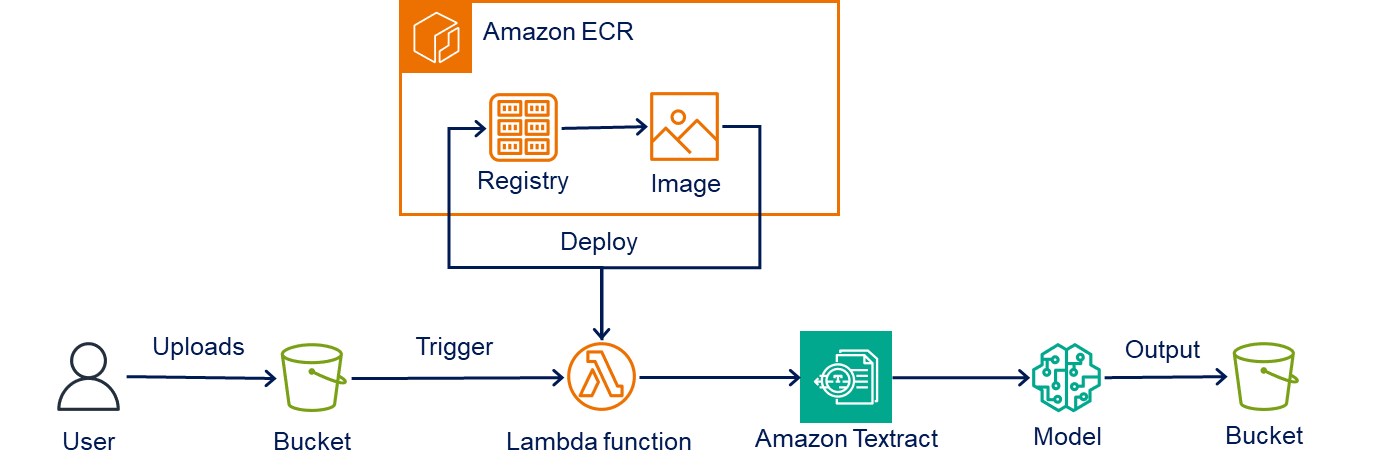
\includegraphics[width=1 \textwidth]{chapters/images/Methods/Deployment/s3_trigger.png}
    \caption{Deployment Workflow of using S3-Bucket to trigger the Lambda}
    \label{fig:s3-trigger-workflow}
\end{figure}



\subsection{Using Rest API to trigger the containerized Lambda\label{workflow_restapi}}

In order to make \acrshort{ml} model available to the end-users over internet the approach discussed in \Cref{s3_deployment} is not sufficient, for instance there is no frontend for the user to interact with and dropping all the results in one bucket can be an issue of managing the results for individuals plus there is a solution for identity and access management is missing. Therefore we proposed the new workflow that combines the frontend and backend as shown in \Cref{fig:API_workflow} so that the \acrshort{ml} model can be served as a web application. In this workflow, the user first reach the frontend where they can interact with the \acrshort{gui}. To make sure the users are who they claim to be, we added one more layer of authentication on top of \acrshort{https}, the authentication flow is shown in \Cref{fig:Authenticationflow}. It starts with users login credentials such as username, email and passwords. The client(frontend) will then send this credential to Amazon Cognito\footnote{\url{https://aws.amazon.com/cognito/}, Accessed: 24.04.2024}. Cognito is a service that is managed by \acrshort{aws} to provide identity and access management. In addition, the cognito offers so called user pool, where we can store all the users. After receiving user's credentials, cognito will compare and check whether if the user is in this user pool or not, if there is no such user exist than it will give unauthorized response and if the user exists in the user pool than cognito send a request to \acrfull{oauth} 2.0, which is a standard designed to allow a website or application to access resources hosted by other web apps on behalf of a user. After processing the request from cognito, \acrshort{oauth} will issue a \acrfull{jwt}\footnote{\url{https://jwt.io/introduction}, Accessed: 24.04.2024}.  \acrshort{jwt} is digitally signed public/private key pair that has been created using cryptographic algorithms like RSA\footnote{\url{https://www.rsa.com/}, Accessed: 24.04.2024}. To have more control over the resources, we kept a lambda authorizer, this authorizer will take this token and check whether if the token is not expired, valid and signed. Based upon the token authenticity, lambda authorizer will create policies, this polices can be used to allow the user to reach various part of the resources. For instance if lambda authorizer identify from the token that the user is admin, than it can give full access to the resources. An example of this polices is described in \Cref{Listing:2}.Once the policy is obtained, it will pass with the request to the resources and user will be considered as a authenticated user. This policies helps to control the usage of the resources, for instance if user have \verb|AUTHORIZED_RESPONSE|, user only can execute action to invoke the \verb|URL_to_Resource| using limited methods (GET, POST) that is defined in backend. 

\begin{figure}[!ht]
    \centering
    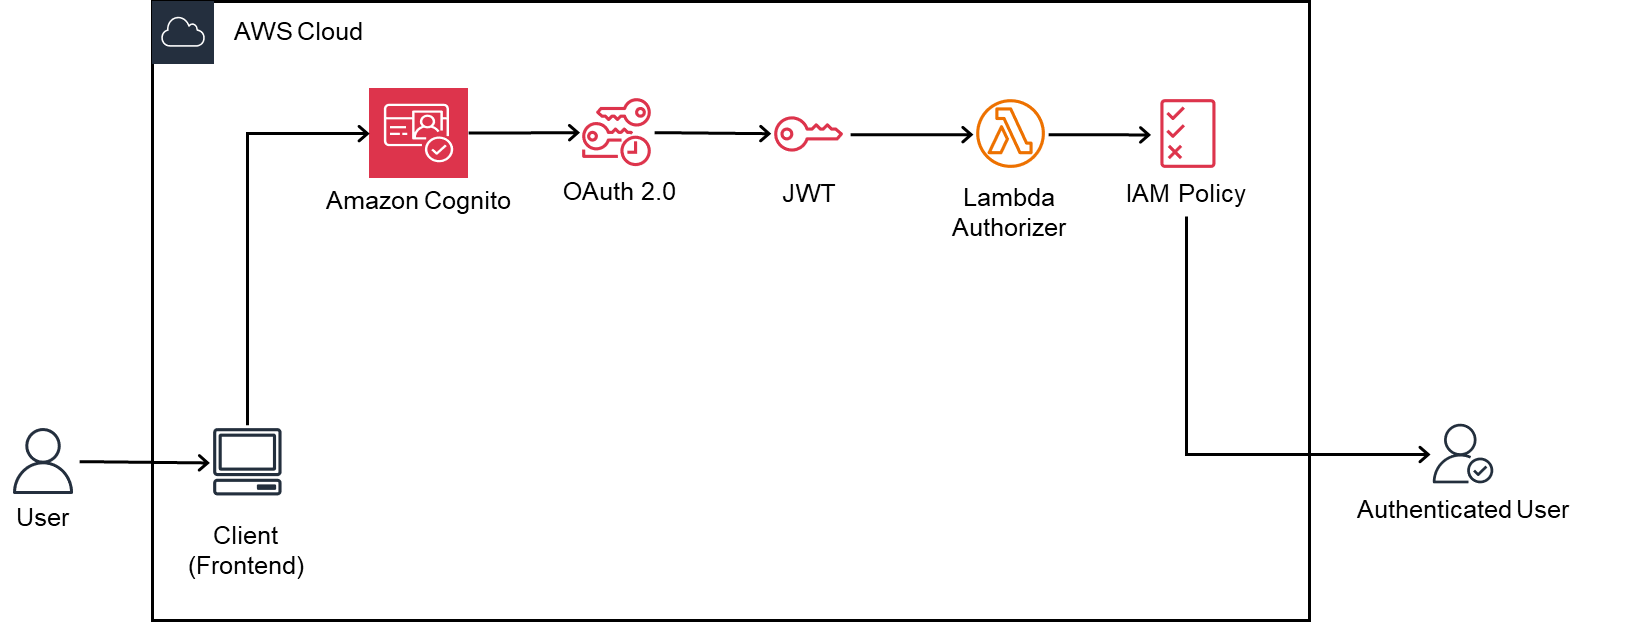
\includegraphics[width=1 \textwidth]{chapters/images/Methods/Deployment/Authentication_flow.png}
    \caption{Authentication flow}
    \label{fig:Authenticationflow}
\end{figure}

\begin{listing}[!ht]

        \begin{minted}{python}
            AUTHORIZED_RESPONSE = {
                "policyDocument": {
                    "Version": "2012-10-17",
                    "Statement": [
                        {
                            "Action": "execute-api:Invoke",
                            "Resource": [f"arn:aws:execute-api:Url_to_Resource"],
                            "Effect":"Allow"
                        }
                    ]
                }
            }

            UNAUTHORIZED_RESPONSE = {
                "policyDocument": {
                    "Version": "2012-10-17",
                    "Statement": [
                        {
                            "Action": "*",
                            "Resource": "*",
                            "Effect": "Deny"
                        }
                    ]
                }
            }
        \end{minted}
    
    \caption{AN Example of IAM policy}
    \label{Listing:2}   
\end{listing}


The backend and frontend implementation is in way that for every API call from the user, the authentication flow (\ref{fig:Authenticationflow}) will be triggered first to check the authenticity of the user. After successful authentication, the user can consume the resources using the frontend as shown in \Cref{fig:API_workflow}. When user sends a document for prediction, first the authentication flow will be initiated and policy will be obtained, this policy will have information like which resource or path to execute, this resources or path depends on the component in the frontend that initiated the request. This Rest API request will trigger a Lambda function deployment process. In this process, the container image will be pulled from \acrshort{ecr} that is having the application's code, \acrshort{ml} model, libraries and all the necessary dependencies to run the application. Once the lambda function is deployed successfully, the document is then sent to AWS Textract to obtain words and bounding boxes from the document which will be letter fed to the model for making a prediction. Once the predictions are ready, the results will be send back to the frontend from where users can see and download the results. 


\begin{figure}[!ht]
    \centering
    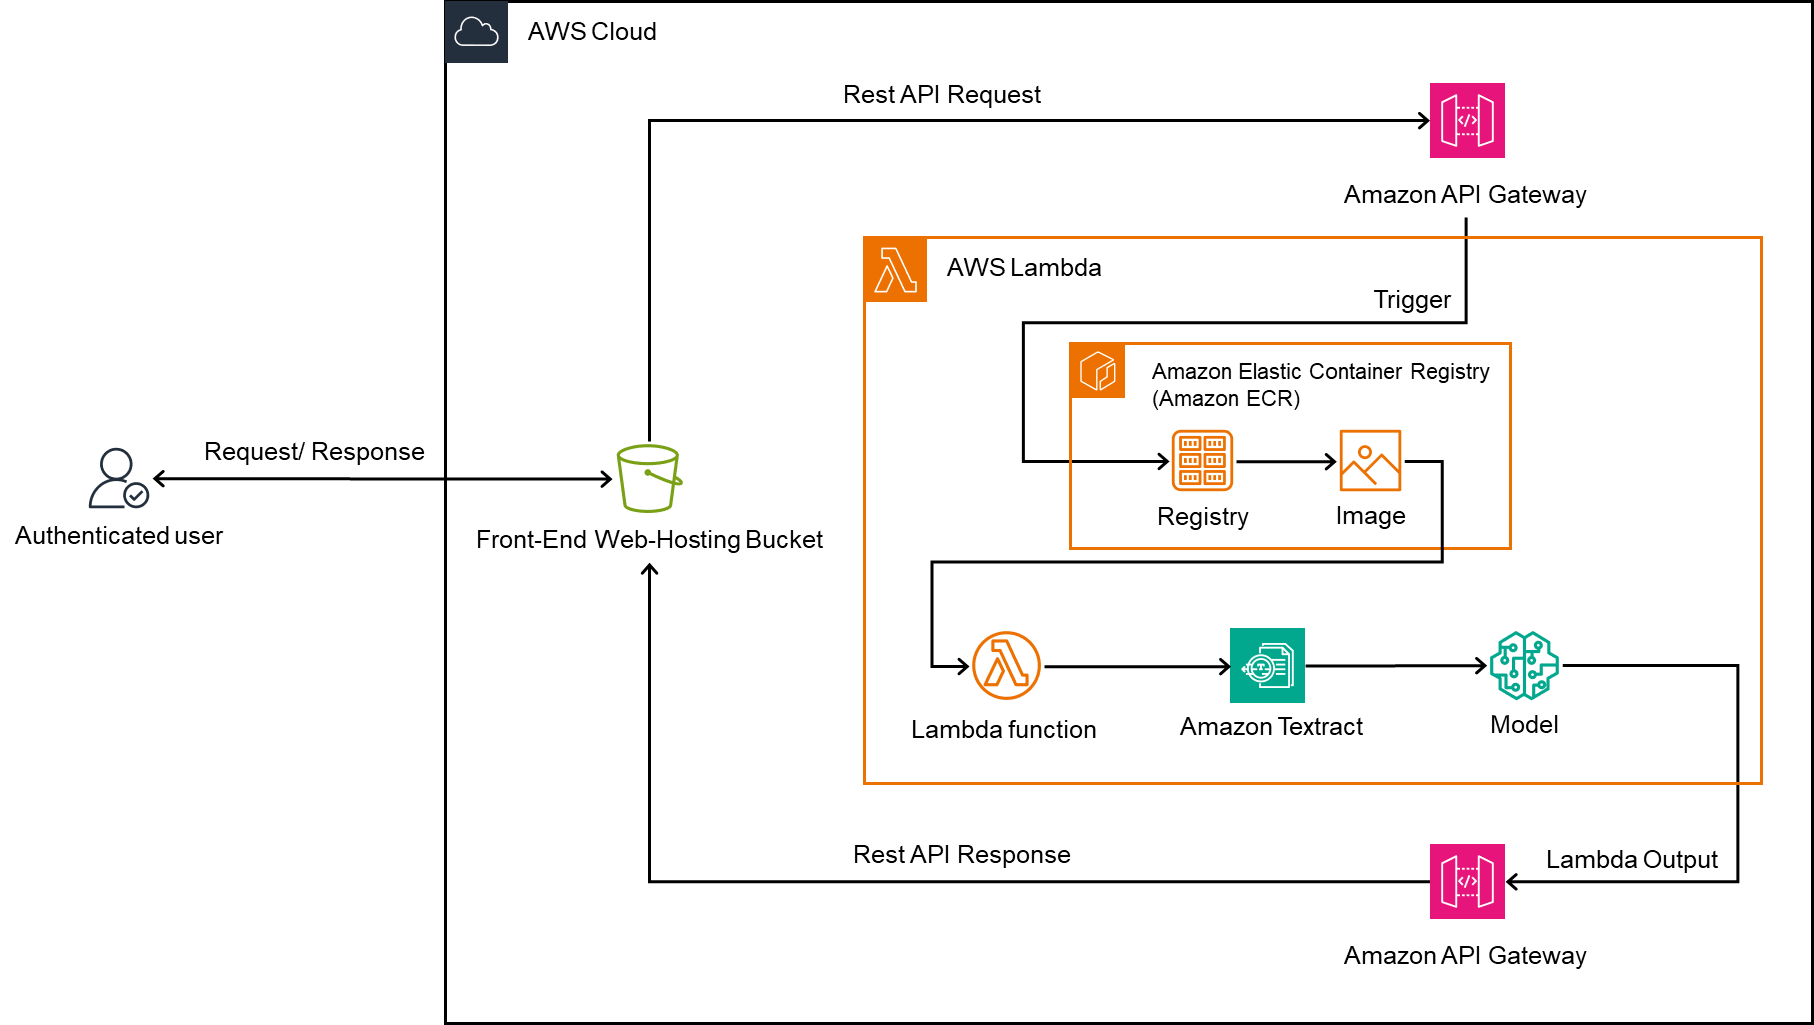
\includegraphics[width=0.95 \textwidth]{chapters/images/Methods/Deployment/Restapi_trigger.png}
    \caption{Using Rest API to trigger the Lambda}
    \label{fig:API_workflow}
\end{figure}

